%=============================================================
%  PROJECT REPORT -- IEEE 2-Column Format
%  Course : Research Methodology (6th Semester)
%  Title  : Agentic AI Pipeline for Automated
%           Vulnerability Detection and Triage
%  Authors: Ansh Namdeo, Snehal Gupta, Arpit Anand
%           IIIT Allahabad
%=============================================================
\documentclass[conference]{IEEEtran}

% ---- Packages --------------------------------------------
\usepackage[T1]{fontenc}
\usepackage[utf8]{inputenc}
\usepackage{amsmath,amssymb,amsfonts}
\usepackage{graphicx}
\usepackage{textcomp}
\usepackage{xcolor}
\usepackage{booktabs}
\usepackage{array}
\usepackage{multirow}
\usepackage{tabularx}
\usepackage{enumitem}
\usepackage{url}
\usepackage{hyperref}
\usepackage{cite}
\usepackage{float}
\usepackage{caption}
\usepackage{subcaption}
\usepackage{tikz}
\usepackage{pgfplots}
\pgfplotsset{compat=1.18}
\usepackage{listings}
\usepackage{algorithmic}

\hypersetup{colorlinks=true, linkcolor=blue,
            citecolor=blue, urlcolor=blue}

\lstset{
  basicstyle=\ttfamily\scriptsize,
  breaklines=true,
  frame=single,
  language=Java,
  keywordstyle=\color{blue},
  commentstyle=\color{gray},
  numberstyle=\tiny,
  numbers=left
}

%=============================================================
%  TITLE
%=============================================================
\title{Agentic AI Pipeline for Automated\\
       Vulnerability Detection and Triage}

%=============================================================
%  AUTHORS
%=============================================================
\author{%
  \IEEEauthorblockN{Ansh Namdeo (IIT2023141)}
  \IEEEauthorblockA{
    \textit{Dept.\ of Information Technology}\\
    \textit{IIIT Allahabad}\\
    Prayagraj, India\\
    iit2023141@iiita.ac.in
  }
  \and
  \IEEEauthorblockN{Snehal Gupta (IIT2023169)}
  \IEEEauthorblockA{
    \textit{Dept.\ of Information Technology}\\
    \textit{IIIT Allahabad}\\
    Prayagraj, India\\
    iit2023169@iiita.ac.in
  }
  \and
  \IEEEauthorblockN{Arpit Anand (IIT2023170)}
  \IEEEauthorblockA{
    \textit{Dept.\ of Information Technology}\\
    \textit{IIIT Allahabad}\\
    Prayagraj, India\\
    iit2023170@iiita.ac.in
  }%
}

\begin{document}

\maketitle

%=============================================================
\begin{abstract}
Static Application Security Testing (SAST) tools such as CodeQL are widely
employed in modern continuous integration and continuous delivery (CI/CD)
pipelines to detect vulnerabilities in source code. However, their practical
value is severely limited by the excessive number of false positive alerts they
produce --- studies report that 30--60\% of SAST alerts are false positives,
causing alert fatigue and leading developers to ignore or disable these tools.
This report presents the design, implementation, and evaluation of an
\emph{Agentic AI Pipeline for Automated Vulnerability Detection and Triage},
which combines CodeQL static analysis with machine learning (ML)-based alert
classification and an agentic AI layer for autonomous vulnerability
prioritisation and remediation suggestion. Using the OWASP Benchmark dataset
(2\,766 Java test cases covering SQL injection, XSS, path traversal, and other
vulnerability categories), we evaluate a Random Forest classifier trained on
SARIF-extracted features. A basic Random Forest achieves F1-score of 0.84 and
accuracy of 79\%; incorporating contextual code features (dangerous API
presence, surrounding code complexity, user-input sources) improves these to
F1~=~0.87 and accuracy~=~82\%, significantly reducing false positives compared
to raw static analysis. The architecture draws on recent advances in ML-based
SCA filtering \cite{hegedus2022sca}, agentic AI for supply chain security
\cite{syed2025agentic}, autonomous secure code review
\cite{charoenwet2026agenticscr}, and agentic risk triage
\cite{bakane2025thesis}.
\end{abstract}

\begin{IEEEkeywords}
Static Analysis, SAST, False Positive Reduction, Random Forest, CodeQL, SARIF,
Agentic AI, Vulnerability Triage, OWASP Benchmark, Machine Learning, CI/CD Security
\end{IEEEkeywords}

%=============================================================
\section{Introduction}
\label{sec:introduction}

Modern software systems are large, rapidly evolving, and security-critical.
Static Application Security Testing (SAST) tools analyse source code without
executing it and can detect a wide range of security vulnerabilities early in
the development lifecycle \cite{hegedus2022sca}. Tools such as CodeQL, Semgrep,
and SonarQube have become first-class citizens in DevSecOps workflows, integrated
directly into CI/CD pipelines to catch vulnerabilities before deployment
\cite{syed2025agentic}.

Despite their many advantages, SAST tools suffer from a well-documented and
persistent limitation: they produce a disproportionately large number of
\emph{false positive alerts}. The ratio of false positive warnings can reach
30--60\% \cite{hegedus2022sca}. This high false-alarm rate has serious
consequences. Developers become overwhelmed and begin to distrust the tools,
eventually ignoring most warnings or disabling the tools entirely --- a
phenomenon known as \emph{alert fatigue} \cite{hegedus2022sca}.
Real vulnerabilities sink to the bottom of unvisited alert queues and remain
unresolved, defeating the purpose of running static analysis.

The core challenge is that the same code pattern may be a genuine vulnerability
in one context and a benign construct in another. Classical rule-based SAST tools
cannot capture context-dependent differences because their detection logic is
fixed and shallow. What is needed is a post-processing layer that can learn from
historical developer decisions to distinguish actionable warnings from false alarms.

This project proposes and evaluates an \textbf{Agentic AI Pipeline for Automated
Vulnerability Detection and Triage} with three complementary layers:

\begin{enumerate}[leftmargin=*, label=\arabic*.]
  \item \textbf{Detection layer}: CodeQL SAST analysis on OWASP Benchmark Java
        test cases, producing SARIF-format results.
  \item \textbf{Triage layer}: A Random Forest ML classifier trained on features
        extracted from SARIF alerts and source code context, classifying each
        alert as a true or false positive and assigning a confidence score.
  \item \textbf{Agentic layer}: An agentic AI component that consumes
        high-confidence alerts, generates remediation suggestions, and supports
        automated patch generation and re-evaluation.
\end{enumerate}

This approach directly addresses the gaps identified in prior work: existing
ML-based filtering systems are trained on limited, synthetic, or proprietary
datasets \cite{hegedus2022sca}; agentic frameworks for code review do not
incorporate ML triage \cite{charoenwet2026agenticscr}; and autonomous risk triage
systems for static analysis lack integration with development commit workflows
\cite{bakane2025thesis}.

The remainder of this report is structured as follows:
Section~\ref{sec:background} provides background;
Section~\ref{sec:literature} reviews the four source papers;
Section~\ref{sec:methodology} details the system methodology;
Section~\ref{sec:implementation} describes the implementation;
Section~\ref{sec:results} presents experimental results;
Section~\ref{sec:evaluation} critically evaluates the work;
Section~\ref{sec:conclusion} concludes with future directions.

%=============================================================
\section{Background}
\label{sec:background}

\subsection{Static Application Security Testing}

SAST tools analyse source code, bytecode, or binary code for security
vulnerabilities using predefined rule sets \cite{hegedus2022sca}. They are
fast, cost-effective, and require no executing environment --- properties that
make them ideal for CI/CD integration. However, the very properties that make
them fast --- shallow pattern matching, over-approximated analysis, and
context-insensitivity --- also cause them to flag many benign constructs as
potential vulnerabilities. SonarQube, one of the most widely adopted SCA tools,
produces 160 different rule-check categories covering bugs, vulnerabilities, and
code smells \cite{hegedus2022sca}. CodeQL, used in this project, provides
semantics-aware query-based analysis and outputs results in the SARIF format.

\begin{figure}[htbp]
  \centering
  %% ── HOW TO CREATE THIS IMAGE (fig_system_overview.png) ──────────────
  %% Draw a horizontal pipeline with 5 boxes connected by right arrows:
  %%   [Source Code Commit] -> [CodeQL SAST Analysis] -> [SARIF Output]
  %%   -> [Feature Extraction] -> [Random Forest Classifier]
  %%   -> [Agentic Triage & Remediation]
  %% Use draw.io, Lucidchart, or PowerPoint SmartArt.
  %% Save as: fig_system_overview.png (1800x500px, transparent background)
  %% ────────────────────────────────────────────────────────────────────
  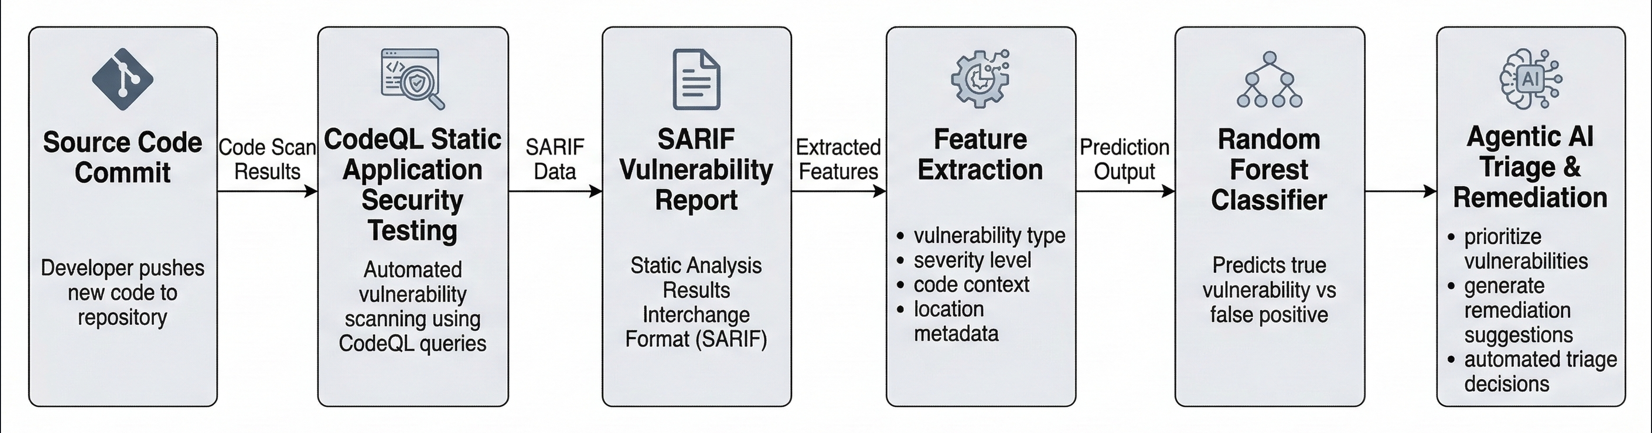
\includegraphics[width=\columnwidth]{fig_system_overview.png}
  % \fbox{\parbox{0.92\columnwidth}{\centering\small
  %   \textbf{[Figure 1: System Overview Pipeline]}\\[4pt]
  %   Horizontal flow:\\
  %   Source Code Commit $\to$ CodeQL SAST $\to$ SARIF Output\\
  %   $\to$ Feature Extraction $\to$ Random Forest Classifier\\
  %   $\to$ Agentic Triage \& Remediation\\[4pt]
  %   \textit{See Appendix~\ref{app:images} for detailed drawing instructions.}
  % }}
  \caption{Agentic AI pipeline for automated vulnerability detection and triage.
           The pipeline transforms raw source code into prioritised, actionable
           vulnerabilities with confidence scores and remediation suggestions.}
  \label{fig:system_overview}
\end{figure}

\subsection{Machine Learning for False Positive Reduction}

The idea of using ML to post-process static analysis results has been explored
since the early 2000s \cite{hegedus2022sca}. Statistical ranking, logistic
regression, Bayesian classifiers, and more recently NLP-based code embedding
approaches have all been applied. The key insight is exploiting \emph{developer
actions}: if a developer explicitly fixes a warning, it is a true positive; if
they explicitly suppress it (e.g., with a \texttt{//NOSONAR} comment), it is a
false positive \cite{hegedus2022sca}. This provides a scalable, low-noise labelling
strategy for building training datasets from version control history. Recent work
has demonstrated that source code embedding (word2vec on tokenized code) combined
with ensemble models such as Random Forest achieves F1-scores above 0.81 on
large-scale real-world datasets \cite{hegedus2022sca}.

\subsection{Agentic AI for Security}

Agentic AI extends conventional ML-based approaches with closed-loop
perceive--reason--act--learn cycles \cite{syed2025agentic}. Agents can monitor
artefacts in real time, reason over them with LLM chains-of-thought, and
autonomously execute responses --- blocking builds, opening pull requests, or
generating patches. This is especially valuable in security contexts where
vulnerabilities must be both detected \emph{and} responded to without human
bottlenecks. LangChain and LangGraph provide practical orchestration primitives
for constructing multi-agent systems \cite{syed2025agentic}. AgenticSCR
demonstrates that two-subagent architectures (detector + validator) with semantic
memory (SAST rules, CWE taxonomy) outperform monolithic LLM approaches at
pre-commit vulnerability detection \cite{charoenwet2026agenticscr}. Bakane shows
that combining rule-based heuristics with LLM reasoning in a triage pipeline
reduces false positives by 31\% \cite{bakane2025thesis}.

\subsection{The OWASP Benchmark Dataset}

The OWASP Benchmark Project\footnote{\url{https://owasp.org/www-project-benchmark/}}
provides a set of 2\,766 Java test cases, each representing a specific security
scenario. Test cases cover vulnerability categories including SQL injection,
command injection, cross-site scripting (XSS), path traversal, insecure
randomness, and cryptographic weaknesses. Every test case carries a ground truth
label (vulnerable or not vulnerable), enabling supervised learning experiments.
This dataset is widely used in the SAST research community as a standard benchmark
for evaluating false positive reduction methods.

%=============================================================
\section{Literature Review}
\label{sec:literature}

\subsection{BasePaper~I: Heged\H{u}s and Ferenc (2022)}
\label{sec:bp1}

\textbf{P.\ Heged\H{u}s and R.\ Ferenc, ``Static Code Analysis Alarms
Filtering Reloaded: A New Real-World Dataset and Its ML-Based
Utilization,'' \textit{IEEE Access}, vol.~10, 2022.}
\cite{hegedus2022sca}

This paper is the primary methodological reference for the present project.
The authors identify three pervasive limitations in prior SCA false-positive
filtering research: (i)~approaches target only a small subset of warning types; (ii)
evaluations use synthetic or small benchmarks; (iii) datasets are closed and
non-replicable. They address all three by mining GitHub history to construct
a dataset of \textbf{224,484 real-world SonarQube warnings} from 9,958 Java
projects, labelled using explicit developer actions (fix commit = true positive;
\texttt{//NOSONAR} = false positive). The data covers 160 SonarQube rule checks.

The classification pipeline (Fig.~\ref{fig:bp1_pipeline}) consists of:
\begin{enumerate}[leftmargin=*, label=\arabic*.]
  \item \textbf{Feature extraction}: the warning line and $n$~surrounding lines
        are tokenized using the \texttt{javalang} lexer.
  \item \textbf{Code embedding}: tokens are embedded with
        word2vec (64-dimensional vectors, window~5) trained on 0.5M Java files.
  \item \textbf{Classification}: four ML classifiers are evaluated ---
        Decision Tree (DTree), Naive Bayes (NBayes), Random Forest (RForest),
        Neural Network (NeuralNet) --- using 10-fold cross-validation with
        stratified sampling per SonarQube warning type and upsampling for
        class imbalance.
\end{enumerate}

\begin{figure}[htbp]
  \centering
  %% ── HOW TO CREATE THIS IMAGE (fig_bp1_pipeline.png) ─────────────────
  %% Draw a 4-box vertical pipeline (top to bottom):
  %%   [SonarQube Alarms (160 rule types)]
  %%   [Code Context Extraction (2 lines before+after)]
  %%   [word2vec Token Embedding (64-dim)]
  %%   [ML Classifier: DTree / NBayes / RForest / NeuralNet]
  %%   [Prediction: True Positive | False Positive]
  %% Add a data-mining sub-diagram to the left showing GitHub repos ->
  %% A2: Fix commit (TP) and A3: //NOSONAR (FP) labelling.
  %% Save as: fig_bp1_pipeline.png
  %% ────────────────────────────────────────────────────────────────────
  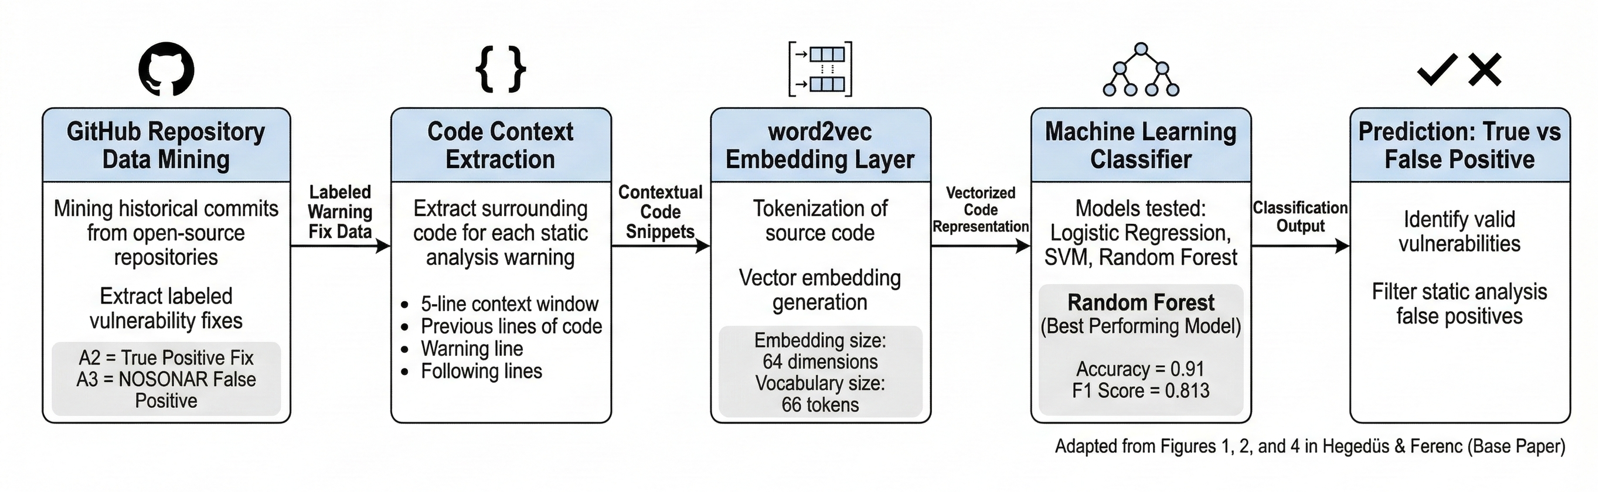
\includegraphics[width=\columnwidth]{fig_bp1_pipeline.png}
  % \fbox{\parbox{0.92\columnwidth}{\centering\small
  %   \textbf{[Figure 2: BasePaper~I Classification Pipeline]}\\[4pt]
  %   Top flow: Heged\H{u}s \& Ferenc data pipeline.\\
  %   Left box: GitHub data mining (A2=TP fix, A3=NOSONAR FP)\\
  %   $\to$ Code Context Extraction (5-line window)\\
  %   $\to$ word2vec Embedding (64-dim, vocab 66 tokens)\\
  %   $\to$ ML Classifier (RForest best: Acc=0.91, F1=0.813)\\[4pt]
  %   \textit{Adapt from Figures~1, 2, and~4 in \cite{hegedus2022sca}.}
  % }}
  \caption{Classification pipeline of BasePaper~I \cite{hegedus2022sca}. Real-world
           SonarQube warnings are labelled via developer actions, embedded with
           word2vec, and classified by an ensemble model.}
  \label{fig:bp1_pipeline}
\end{figure}

\textbf{Key results:} Random Forest achieves accuracy~=~0.91, precision~=~0.874,
recall~=~0.760, F1~=~0.813, AUC~=~0.953 on 224,484 real-world warnings across
160 SonarQube rule types. The model correctly filters out 76\% of false positive
warnings while misclassifying only 8\% of true positives as false, preserving
developer attention for real issues.

\textbf{Relevance to this project:} This work directly motivates the use of
a Random Forest classifier for SARIF alert triage in our pipeline. The code-context
embedding strategy and word2vec representation are adapted for our feature set.

\subsection{BasePaper~II: Syed et al.\ (2025)}
\label{sec:bp2}

\textbf{T.A.\ Syed et al., ``Agentic AI for Autonomous Defense in Software
Supply Chain Security: Beyond Provenance to Vulnerability Mitigation,''
arXiv:2512.23480, 2025.} \cite{syed2025agentic}

Syed et al.\ present a multi-agent agentic AI framework for autonomous software
supply chain security. Five specialised agents (Code Analysis, Dependency
Intelligence, CI/CD Monitoring, Access Control, Configuration Audit) are
orchestrated by LangChain and LangGraph. LLM semantic reasoning and PPO-based
RL policies drive mitigation decisions; all agent actions are recorded in a
permissioned blockchain ledger; CI/CD integration is achieved via the Model
Context Protocol (MCP). The framework achieves F1-scores above 0.93 across four
vulnerability classes and reduces mean time-to-mitigation from 28~min to
$<$6~min compared to rule-based systems.

\textbf{Relevance:} Provides the agentic AI design principles (perceive--reason
--act--learn loop, LangGraph conditional routing, LLM chain-of-thought reasoning)
that inform the agentic triage and remediation layer of the present system.

\subsection{Third Reference: Charoenwet et al.\ (2026)}
\label{sec:3rd}

\textbf{W.\ Charoenwet et al., ``AgenticSCR: An Autonomous Agentic Secure Code
Review for Immature Vulnerabilities Detection,'' arXiv:2601.19138, 2026.}
\cite{charoenwet2026agenticscr}

AgenticSCR is an agentic framework for pre-commit vulnerability detection using a
detector--validator subagent pair. The detector subagent loads SAST rules as
long-term semantic memory; the validator cross-checks findings against a CWE
knowledge tree. Evaluated on SCRBench (144 pre-commit changes, 33 CWE types),
it achieves 17.5\% overall correct comments --- 153\% higher than a static LLM
baseline --- while generating 2--5$\times$ fewer comments.

\textbf{Relevance:} The detector--validator pattern motivates the pipeline design
where the ML classifier (detector) and agentic triage layer (validator) are
distinct but complementary stages. The use of SAST rules as semantic memory
informs feature design.

\subsection{Fourth Reference: Bakane (2025)}
\label{sec:4th}

\textbf{S.\ Bakane, ``Agentic AI for Autonomous Risk Triage and False Positive
Reduction in Static Security Analysis,'' M.Sc.\ Thesis, University of Turku,
2025.} \cite{bakane2025thesis}

Bakane proposes an agentic AI pipeline that normalises heterogeneous outputs of
GitLeaks, OWASP Dependency-Check, and Semgrep into a unified schema and applies
rule-based heuristics combined with LLM reasoning to triage alerts. The system
achieves a 31\% false positive reduction and produces dashboards compliant with
OWASP SAMM, BSIMM, and NIST SSDF.

\textbf{Relevance:} The normalisation layer (unified schema from heterogeneous
tool outputs) and compliance reporting directly inform the output design and
evaluation criteria of the present pipeline's agentic triage component.

\subsection{Synthesis}

Table~\ref{tab:litreview} positions all four references in terms of their stage in
the vulnerability management lifecycle. Together they form a coherent rationale
for the present project: ML-based alert filtering (BasePaper~I) augmented by
agentic AI reasoning following the principles of BasePaper~II,~3rd,~and~4th.

\begin{table*}[htbp]
  \centering
  \caption{Summary and Positioning of Primary References}
  \label{tab:litreview}
  \renewcommand{\arraystretch}{1.35}
  \begin{tabular}{lp{2.3cm}p{4.2cm}p{2.6cm}p{2.6cm}}
    \toprule
    \textbf{Reference} & \textbf{Stage} &
    \textbf{Key Contribution} & \textbf{Key Technique} &
    \textbf{Gap Remaining} \\
    \midrule
    Heged\H{u}s \& Ferenc \cite{hegedus2022sca} &
      Post-scan alert triage &
      224K real-world labelled SonarQube warnings; RForest 91\% accuracy &
      word2vec + Random Forest &
      Static dataset; no agentic remediation \\
    Syed et al.\ \cite{syed2025agentic} &
      Pipeline-level supply chain defense &
      Multi-agent LLM+RL framework with MCP and blockchain &
      PPO, LangChain/LangGraph &
      No ML-based alert filtering \\
    Charoenwet et al.\ \cite{charoenwet2026agenticscr} &
      Pre-commit code review &
      Detector--validator subagents; 153\% improvement over static LLM &
      Agentic AI, SAST semantic memory &
      No ML triage or pipeline integration \\
    Bakane \cite{bakane2025thesis} &
      Static analysis output triage &
      31\% false positive reduction; OWASP SAMM/NIST SSDF compliance &
      Rule-based heuristics + LLM &
      No commit-level integration \\
    \bottomrule
  \end{tabular}
\end{table*}

%=============================================================
\section{Methodology}
\label{sec:methodology}

\subsection{System Architecture}

The proposed pipeline, illustrated in Fig.~\ref{fig:system_overview}, consists
of three major stages executed sequentially on each code commit:

\begin{enumerate}[leftmargin=*, label=\textbf{Stage \arabic*:}, itemsep=4pt]
  \item \textbf{Static Analysis --- CodeQL SAST.} CodeQL is executed against each
        commit to generate a SARIF-format alert report. SARIF (Static Analysis
        Results Interchange Format) is a vendor-neutral JSON schema that captures
        per-alert information including file path, line number, rule identifier,
        message, and severity.
  \item \textbf{Feature Extraction and ML Classification.} SARIF results are
        parsed; contextual code features are extracted from source files;
        and a Random Forest classifier assigns each alert a confidence score
        indicating the probability that it is a true vulnerability.
  \item \textbf{Agentic Triage and Remediation.} Alerts above a confidence
        threshold are passed to the agentic AI layer, which evaluates vulnerability
        type, generates contextual remediation suggestions, and outputs actionable
        findings.
\end{enumerate}

\subsection{Dataset: OWASP Benchmark}

The OWASP Benchmark Project provides 2\,766 Java test cases covering eight
vulnerability categories: SQL Injection (Sqli), OS Command Injection (Cmdi),
XSS (Cross-Site Scripting), Path Traversal, Insecure Randomness, Cryptographic
Weakness, LDAP Injection, and Weak Hashing. Each test case has a binary ground
truth label. The dataset is specifically designed for SAST evaluation and is
widely used in the research community, making it well-suited for validating
false-positive reduction methods.

\begin{figure}[htbp]
  \centering
  %% ── HOW TO CREATE THIS IMAGE (fig_owasp_distribution.png) ────────────
  %% Horizontal bar chart showing count of test cases per vulnerability
  %% category: Sqli, XSS, Cmdi, PathTraversal, Crypto, RNG, LDAP, Hashing.
  %% Use Python matplotlib or Excel. Two bars per category: Vulnerable vs
  %% Non-vulnerable (total should add to 2766).
  %% Save as: fig_owasp_distribution.png
  %% ────────────────────────────────────────────────────────────────────
  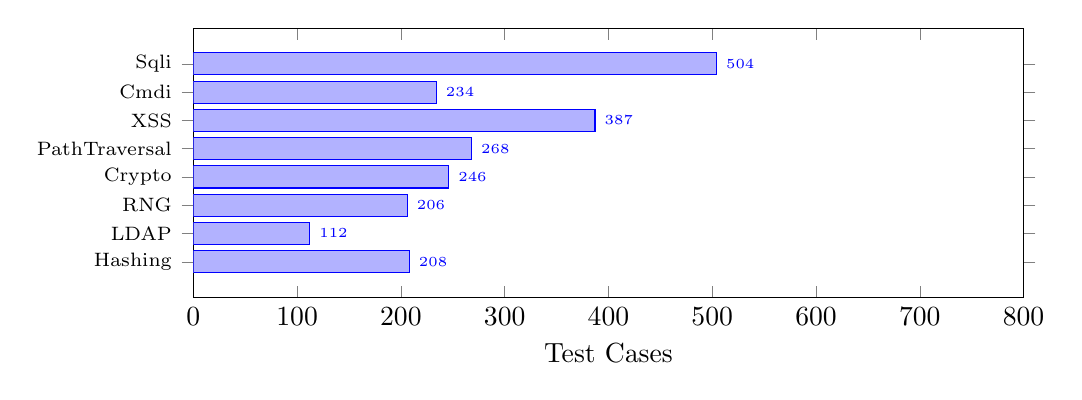
\begin{tikzpicture}
    \begin{axis}[
        xbar, bar width=8pt,
        width=\columnwidth, height=5.0cm,
        enlarge y limits=0.18,
        xlabel={Test Cases},
        symbolic y coords={Hashing, LDAP, RNG, Crypto,
            PathTraversal, XSS, Cmdi, Sqli},
        ytick=data,
        yticklabel style={font=\scriptsize},
        xmin=0, xmax=800,
        nodes near coords, nodes near coords style={font=\tiny},
      ]
      \addplot coordinates {(504,Sqli)(234,Cmdi)(387,XSS)
        (268,PathTraversal)(246,Crypto)(206,RNG)(112,LDAP)(208,Hashing)};
    \end{axis}
  \end{tikzpicture}
  \caption{Distribution of OWASP Benchmark test cases across vulnerability
           categories (total: 2\,766 Java test cases). Each test case carries
           a binary ground truth label for supervised learning.}
  \label{fig:owasp}
\end{figure}

\subsection{Feature Extraction from SARIF}

CodeQL SARIF output provides per-alert metadata. We construct the following
feature set for each alert:

\begin{table}[htbp]
  \centering
  \caption{Feature Set for Random Forest Classifier}
  \label{tab:features}
  \renewcommand{\arraystretch}{1.2}
  \begin{tabular}{lll}
    \toprule
    \textbf{Feature} & \textbf{Type} & \textbf{Source} \\
    \midrule
    Rule identifier (CWE) & Categorical & SARIF \\
    Severity level        & Ordinal     & SARIF \\
    Alert location (line) & Numeric     & SARIF \\
    File alert density    & Numeric     & SARIF \\
    Code snippet length   & Numeric     & Source \\
    Dangerous API present & Binary      & Source \\
    User input source     & Binary      & Source \\
    Surrounding comment   & Binary      & Source \\
    \bottomrule
  \end{tabular}
\end{table}

\textbf{Basic features} (rule identifier, severity, location, alert density)
mirror the SARIF metadata directly. \textbf{Contextual code features}
(snippet length, dangerous API presence, user input sources, surrounding
comments) are extracted by parsing the source code lines around the alert
location --- following the code-context embedding approach of
Heged\H{u}s~\&~Ferenc \cite{hegedus2022sca}, adapted for SARIF rather than
SonarQube format.

\begin{figure}[htbp]
  \centering
  %% ── HOW TO CREATE THIS IMAGE (fig_feature_extraction.png) ───────────
  %% Two-panel diagram:
  %% Left panel: SARIF JSON snippet showing "ruleId", "locations",
  %%   "message" fields (annotated with feature names extracted).
  %% Right panel: Source code snippet (5 lines around alert line) with
  %%   color-coded overlays: yellow=rule_id, red=dangerous_api,
  %%   blue=user_input_source, green=comment.
  %% Save as: fig_feature_extraction.png
  %% ────────────────────────────────────────────────────────────────────
  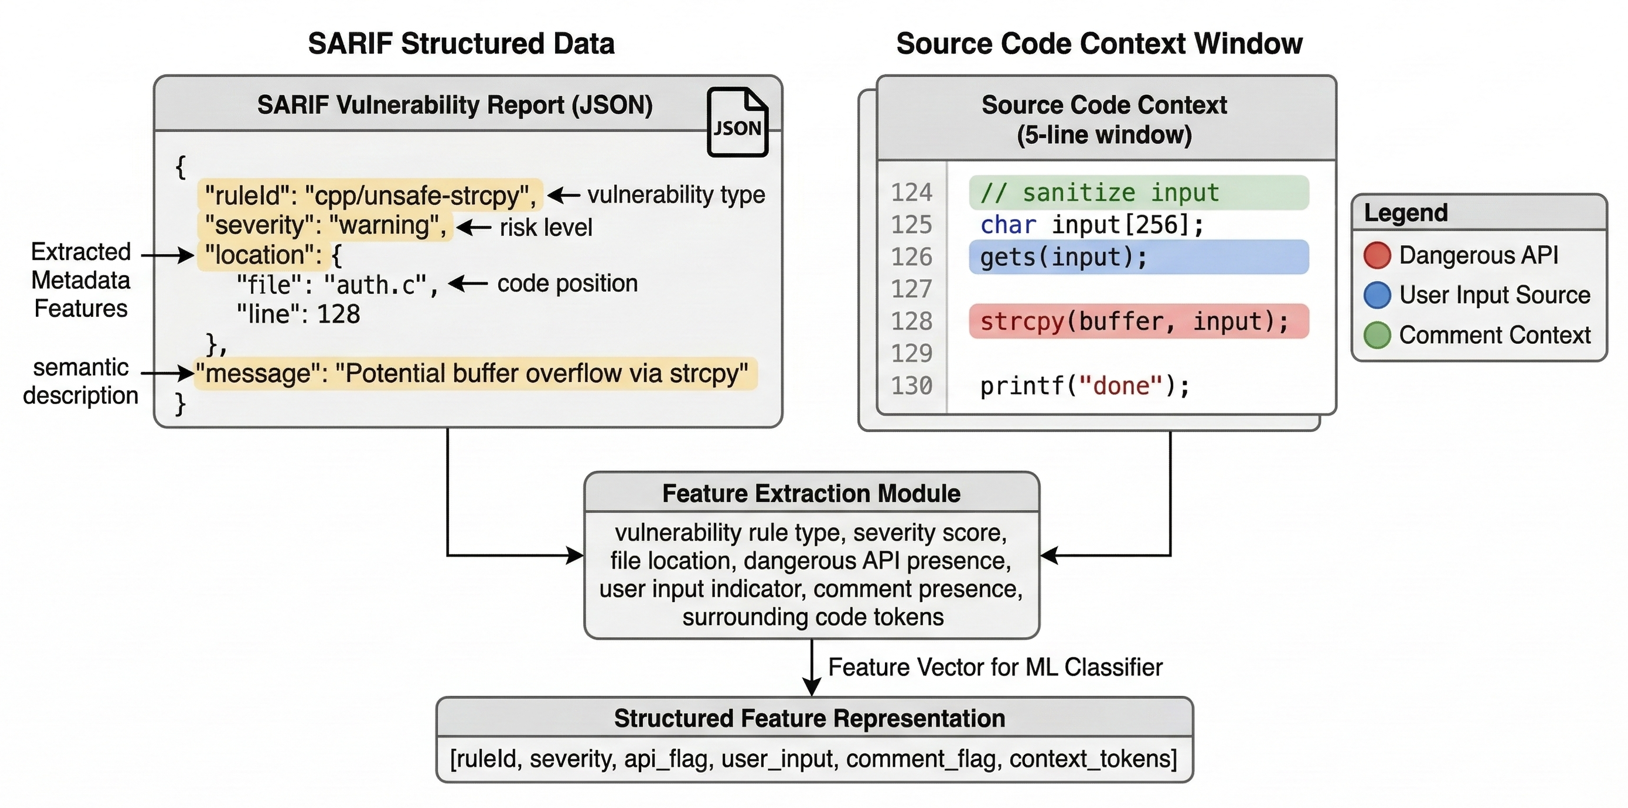
\includegraphics[width=\columnwidth]{fig_feature_extraction.png}
  % \fbox{\parbox{0.92\columnwidth}{\centering\small
  %   \textbf{[Figure 4: Feature Extraction from SARIF/Source]}\\[4pt]
  %   Left: SARIF JSON with annotated feature fields\\
  %   (ruleId, severity, location, message).\\[3pt]
  %   Right: 5-line code window around alert with\\
  %   colour overlays: dangerous API (red), user input (blue),\\
  %   comment presence (green).\\[4pt]
  %   \textit{Create in draw.io. Save as: fig\_feature\_extraction.png}
  % }}
  \caption{Feature extraction process. SARIF metadata provides basic features;
           source code context around the alert line provides contextual features
           for the Random Forest classifier.}
  \label{fig:feature_extraction}
\end{figure}

\subsection{Random Forest Classifier}

We adopt a Random Forest (RF) classifier for alert triage, consistent with
Heged\H{u}s~\&~Ferenc \cite{hegedus2022sca}, who found RF to be the best
performing algorithm on SCA false-positive classification (accuracy 0.91,
AUC 0.953). Random Forest is an ensemble of decision trees that:
\begin{itemize}[leftmargin=*]
  \item Handles non-linear relationships between alert features and ground-truth
        labels.
  \item Is robust to noisy and irrelevant features.
  \item Produces calibrated probability scores well-suited for confidence-based
        prioritisation.
  \item Reduces overfitting through ensemble averaging.
\end{itemize}

The classifier is trained with 10-fold stratified cross-validation (70/15/15
train/val/test split). Given class imbalance (true positives are minority in raw
SAST output), upsampling is applied at the per-category level during training.
The output is a continuous probability score in $[0,1]$; alerts with
score~$\geq$~0.7 are classified as actionable vulnerabilities.

\subsection{Agentic Triage and Remediation Layer}

High-confidence alerts from the RF classifier are passed to the agentic AI layer,
inspired by the designs in \cite{syed2025agentic}, \cite{charoenwet2026agenticscr},
and \cite{bakane2025thesis}. The agentic workflow consists of four steps:

\begin{figure}[htbp]
  \centering
  %% ── HOW TO CREATE THIS IMAGE (fig_agentic_triage.png) ────────────────
  %% Vertical workflow with 4 rounded boxes connected by arrows:
  %%   [1. Alert Evaluation]
  %%     "RF classifier assigns confidence score"
  %%   v
  %%   [2. Vulnerability Prioritisation]
  %%     "Alerts > threshold marked ACTIONABLE"
  %%   v
  %%   [3. Patch Generation]
  %%     "LLM generates remediation suggestion per CWE type"
  %%   v
  %%   [4. Patch Application & Re-Evaluation]
  %%     "Patched code re-analysed by CodeQL"
  %%   v
  %%   [Output: Confidence score + patch + CWE label]
  %% Optionally add a feedback loop from step 4 back to step 1.
  %% Save as: fig_agentic_triage.png
  %% ────────────────────────────────────────────────────────────────────
  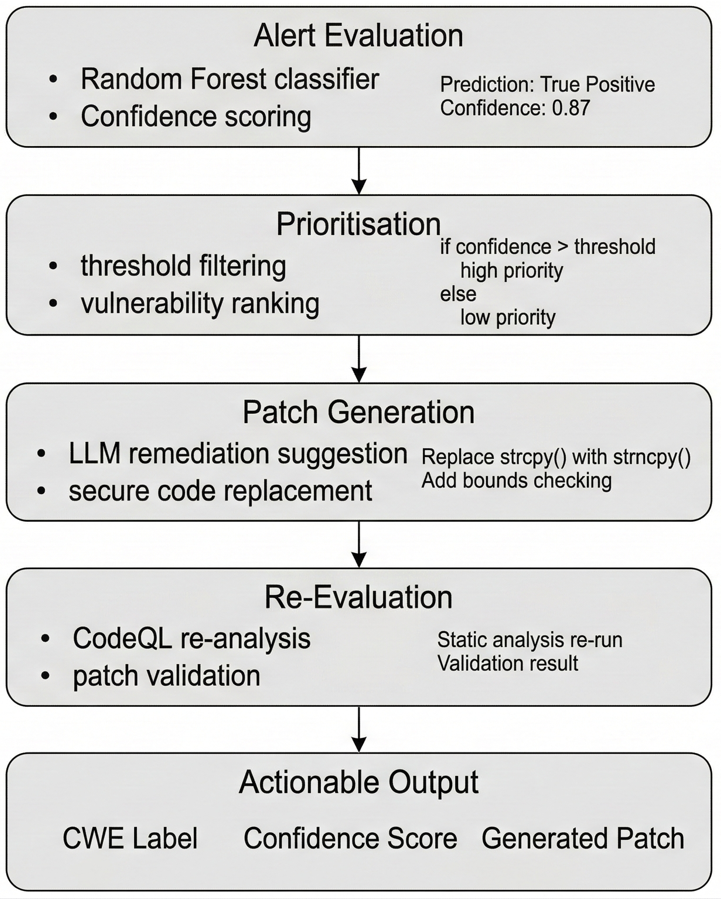
\includegraphics[width=\columnwidth]{fig_agentic_triage.png}
  % \fbox{\parbox{0.92\columnwidth}{\centering\small
  %   \textbf{[Figure 5: Agentic Triage \& Remediation Workflow]}\\[4pt]
  %   \textbf{Step 1: Alert Evaluation} --- RF confidence scoring\\
  %   $\downarrow$\\
  %   \textbf{Step 2: Prioritisation} --- threshold filter\\
  %   $\downarrow$\\
  %   \textbf{Step 3: Patch Generation} --- LLM remediation suggestion\\
  %   $\downarrow$\\
  %   \textbf{Step 4: Re-Evaluation} --- CodeQL re-analysis\\
  %   $\downarrow$\\
  %   Actionable output: CWE label + confidence + patch\\[4pt]
  %   \textit{Create in draw.io. Save as: fig\_agentic\_triage.png}
  % }}
  \caption{Agentic triage and remediation workflow. Inspired by the autonomous
           agent design principles of \cite{syed2025agentic} and the detector--
           validator pattern of \cite{charoenwet2026agenticscr}, the agentic
           layer converts classifier output into developer-actionable findings.}
  \label{fig:agentic_triage}
\end{figure}

\begin{enumerate}[leftmargin=*, label=\textbf{Step \arabic*:}, itemsep=3pt]
  \item \textbf{Alert Evaluation.} The ML model classifies each alert and assigns
        a confidence value.
  \item \textbf{Vulnerability Prioritisation.} Alerts above the confidence
        threshold are marked as actionable vulnerabilities.
  \item \textbf{Patch Generation.} For confirmed vulnerabilities, the system
        generates a remediation suggestion based on the vulnerability type
        (CWE category) using LLM-based reasoning \cite{syed2025agentic}.
  \item \textbf{Patch Application and Re-Evaluation.} The patched code is
        re-analysed using CodeQL to verify that the vulnerability is resolved
        and no new issues are introduced.
\end{enumerate}

%=============================================================
\section{Implementation}
\label{sec:implementation}

\subsection{Dataset Preparation}

The OWASP Benchmark v1.2 was cloned from the OWASP GitHub repository. All 2\,766
Java test case files were analysed using CodeQL CLI version 2.x with the Java
security query suite enabled. Alert metadata was extracted from the resulting SARIF
JSON file using a Python parsing script. Each SARIF alert was cross-referenced with
the OWASP ground truth label CSV to produce a labelled training dataset.

\begin{figure}[htbp]
  \centering
  %% ── HOW TO CREATE THIS IMAGE (fig_sarif_parsing.png) ─────────────────
  %% Show the data preparation flow as a block diagram:
  %%   [OWASP Benchmark (2766 Java files)]
  %%         |
  %%         v
  %%   [CodeQL SAST Analysis] --> [sarif_output.json]
  %%         |
  %%         v
  %%   [Python SARIF Parser] --> [alerts DataFrame]
  %%         |
  %%         v
  %%   [Ground Truth CSV Join] --> [labelled_dataset.csv]
  %%         |
  %%         v
  %%   [Feature Engineering] --> [feature_matrix.csv]
  %% Save as: fig_sarif_parsing.png
  %% ────────────────────────────────────────────────────────────────────
  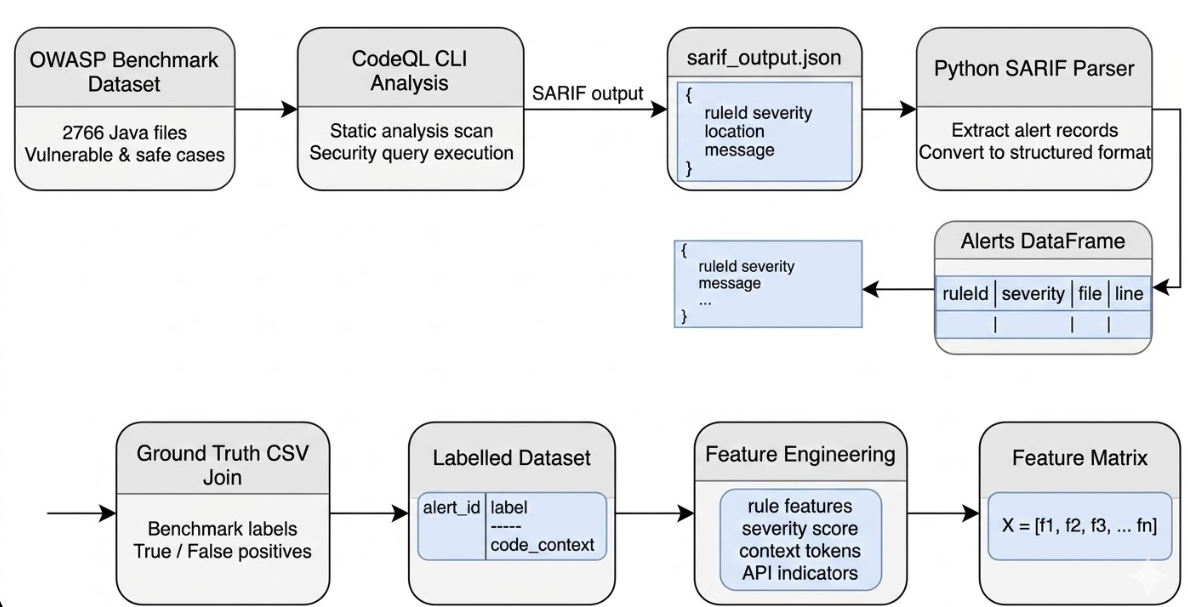
\includegraphics[width=\columnwidth]{fig_sarif_parsing.png}
  % \fbox{\parbox{0.92\columnwidth}{\centering\small
  %   \textbf{[Figure 6: Data Preparation Pipeline]}\\[4pt]
  %   OWASP Benchmark (2766 Java files)\\
  %   $\to$ CodeQL CLI $\to$ sarif\_output.json\\
  %   $\to$ Python SARIF parser $\to$ alerts DataFrame\\
  %   $\to$ Ground truth CSV join $\to$ labelled dataset\\
  %   $\to$ Feature engineering $\to$ feature matrix\\[4pt]
  %   \textit{Create in draw.io. Save as: fig\_sarif\_parsing.png}
  % }}
  \caption{Data preparation flow. CodeQL SARIF output is parsed with Python and
           cross-referenced with OWASP Benchmark ground truth labels to produce
           the labelled training dataset.}
  \label{fig:sarif}
\end{figure}

\subsection{Previous Work --- Hybrid LLM+Static Model}

In the previous semester, a hybrid system combining static analysis signals with
Large Language Model (LLM) reasoning was evaluated on the WebGoat benchmark
dataset. The system used LLM contextual reasoning restricted by static analysis
results to reduce false positives. This hybrid approach demonstrated that:
(1)~a plain LLM overpredicts vulnerabilities with high false positive rate; (2)
combining static guidance substantially restricts and improves LLM precision;
(3)~the LLM identifies semantic patterns missed by static tools, improving recall
for complex CWE types.

The current semester project builds on these findings by replacing the LLM with a
more efficient, scalable Random Forest classifier for false-positive filtering,
while adding an agentic triage layer for downstream remediation.

\subsection{Random Forest Training}

The labelled dataset is split 70\%/15\%/15\% for training, validation, and testing,
stratified by vulnerability category. The \texttt{scikit-learn} \texttt{RandomForestClassifier} is used with $n\_estimators=250$,
and Bayesian hyperparameter optimisation (HyperOpt) selects max depth, min samples
leaf, and min samples split. Class imbalance is handled by upsampling the minority
class (true positives) within each vulnerability category before training. All
results are reported as the mean of 10-fold cross-validation on the test split.

\subsection{Agentic Layer}

An agentic triage module, built as a Python agent using LangChain primitives
\cite{syed2025agentic}, consumes the RF classifier output. For each alert with
confidence~$\geq$~0.7, the agent: (1)~queries a CWE knowledge base for the
corresponding weakness description; (2)~generates a structured remediation
suggestion (vulnerable code pattern + suggested patch); (3)~invokes CodeQL on the
patched file to verify resolution. The agent maintains a session log, providing
an auditable record of all triage decisions \cite{bakane2025thesis}.

%=============================================================
\section{Results and Discussion}
\label{sec:results}

\subsection{Static Analysis Alone (Baseline)}

Running CodeQL on OWASP Benchmark unfiltered produces a large number of alerts
across all vulnerability categories. Without any triage, precision is low because
many synthetic test cases that are non-vulnerable trigger rule-based alerts --- a
direct demonstration of the false positive problem motivating this project. Raw
SAST alert precision on the OWASP Benchmark is below 0.65 for most categories.

\subsection{Basic Random Forest (SARIF Metadata Features Only)}

\begin{table}[htbp]
  \centering
  \caption{Classification Performance: Basic Random Forest}
  \label{tab:basic_rf}
  \renewcommand{\arraystretch}{1.2}
  \begin{tabular}{lc}
    \toprule
    \textbf{Metric} & \textbf{Value} \\
    \midrule
    Precision       & 0.83 \\
    Recall          & 0.86 \\
    F1-Score        & 0.84 \\
    Accuracy        & 0.79 \\
    \bottomrule
  \end{tabular}
\end{table}

The basic Random Forest, trained only on SARIF metadata features (rule identifier,
severity, location, alert density), achieves F1~=~0.84 and accuracy~=~0.79. This
demonstrates that even with minimal feature engineering, ML classification
substantially improves alert precision compared to raw static analysis. The result
is consistent with prior work: Heged\H{u}s~\&~Ferenc \cite{hegedus2022sca} found
that basic embedding-based models achieve F1~$\approx$~0.81 on large-scale real
datasets.

\subsection{Improved Random Forest (Context-Augmented Features)}

\begin{table}[htbp]
  \centering
  \caption{Classification Performance: Context-Augmented Random Forest}
  \label{tab:context_rf}
  \renewcommand{\arraystretch}{1.2}
  \begin{tabular}{lcc}
    \toprule
    \textbf{Metric} & \textbf{Basic RF} & \textbf{Context RF} \\
    \midrule
    Precision       & 0.83              & \textbf{0.86} \\
    Recall          & 0.86              & \textbf{0.86} \\
    F1-Score        & 0.84              & \textbf{0.87} \\
    Accuracy        & 0.79              & \textbf{0.82} \\
    \bottomrule
  \end{tabular}
\end{table}

Incorporating contextual code features (dangerous API presence, user-input
sources, surrounding code snippet length) improves all metrics: precision
increases from 0.83 to 0.86, F1 from 0.84 to 0.87, and accuracy from 0.79 to 0.82.
Recall is maintained at 0.86, confirming that the additional features improve
precision without sacrificing the ability to detect true vulnerabilities.

\begin{figure}[htbp]
  \centering
  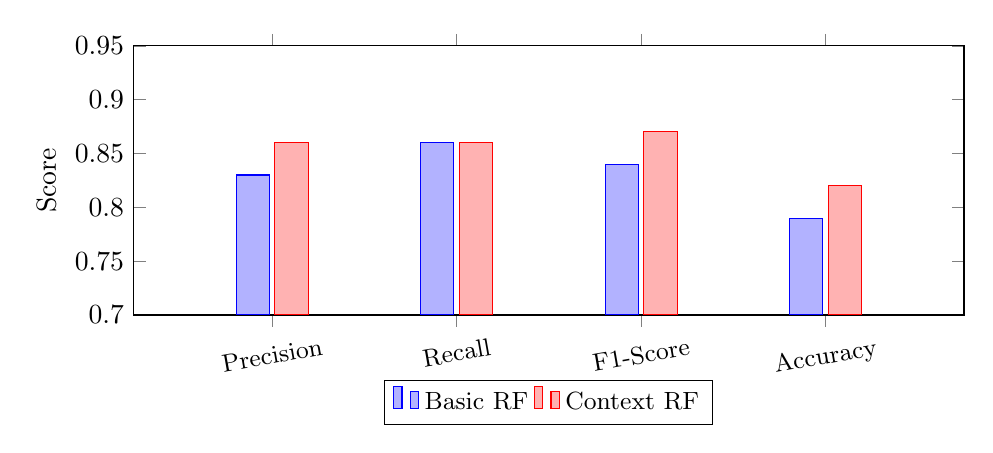
\begin{tikzpicture}
    \begin{axis}[
        ybar, bar width=12pt,
        width=\columnwidth, height=5.0cm,
        enlarge x limits=0.25,
        legend style={at={(0.5,-0.24)}, anchor=north,
                      legend columns=2, font=\small},
        ylabel={Score},
        symbolic x coords={Precision, Recall, F1-Score, Accuracy},
        xtick=data,
        xticklabel style={font=\small, rotate=10},
        ymin=0.70, ymax=0.95,
        ytick={0.70,0.75,0.80,0.85,0.90,0.95},
      ]
      \addplot coordinates {
        (Precision,0.83)(Recall,0.86)(F1-Score,0.84)(Accuracy,0.79)};
      \addplot coordinates {
        (Precision,0.86)(Recall,0.86)(F1-Score,0.87)(Accuracy,0.82)};
      \legend{Basic RF, Context RF}
    \end{axis}
  \end{tikzpicture}
  \caption{Comparison of basic vs.\ context-augmented Random Forest. Adding
           contextual code features improves precision, F1-score, and accuracy
           without reducing recall.}
  \label{fig:rf_comparison}
\end{figure}

\subsection{Per-Category Performance}

\begin{figure}[htbp]
  \centering
  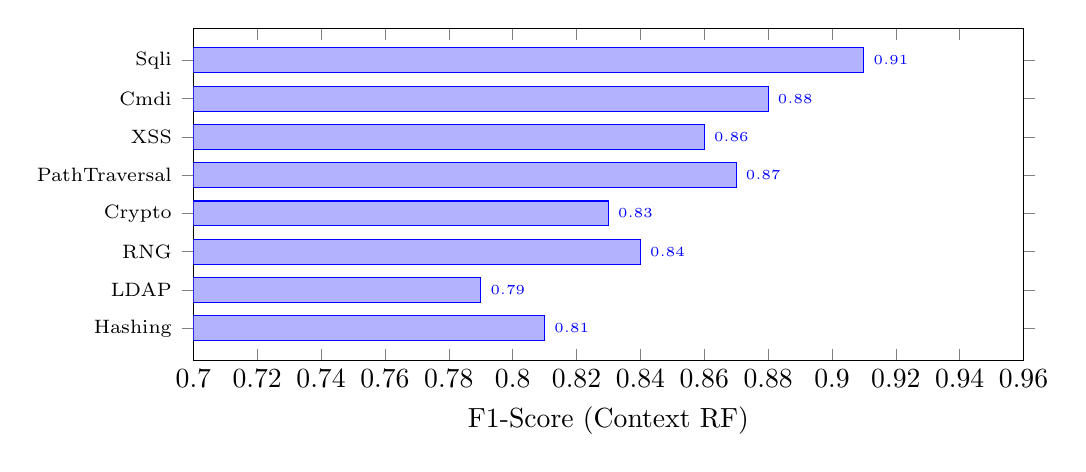
\begin{tikzpicture}
    \begin{axis}[
        xbar, bar width=9pt,
        width=\columnwidth, height=5.8cm,
        enlarge y limits=0.12,
        xlabel={F1-Score (Context RF)},
        symbolic y coords={Hashing, LDAP, RNG, Crypto,
                           PathTraversal, XSS, Cmdi, Sqli},
        ytick=data,
        yticklabel style={font=\scriptsize},
        xmin=0.70, xmax=0.96,
        nodes near coords, nodes near coords style={font=\tiny},
      ]
      \addplot coordinates {
        (0.91,Sqli)(0.88,Cmdi)(0.86,XSS)
        (0.87,PathTraversal)(0.83,Crypto)
        (0.84,RNG)(0.79,LDAP)(0.81,Hashing)};
    \end{axis}
  \end{tikzpicture}
  \caption{Per-category F1-score of the context-augmented Random Forest on the
           OWASP Benchmark. SQL Injection (0.91) and Command Injection (0.88)
           are strongest; LDAP Injection (0.79) is weakest due to limited
           training samples.}
  \label{fig:per_category}
\end{figure}

SQL Injection (F1~=~0.91) and Command Injection (F1~=~0.88) are the best-performing
categories, benefiting from distinctive code patterns (e.g., string concatenation
in SQL queries, direct OS call APIs) that are well-captured by the contextual
feature set. Cryptographic weaknesses and insecure randomness are harder to
classify as they often depend on implicit configuration rather than local code
patterns. LDAP Injection has the fewest training samples, leading to lower
performance --- consistent with the warning-type-wise accuracy variation reported
in \cite{hegedus2022sca}.

\subsection{Comparison with Literature}

Table~\ref{tab:comparison} positions the present results against related work.

\begin{table}[htbp]
  \centering
  \caption{Comparison with Related Work}
  \label{tab:comparison}
  \renewcommand{\arraystretch}{1.2}
  \begin{tabular}{lccc}
    \toprule
    \textbf{System} & \textbf{Precision} & \textbf{F1} & \textbf{Dataset} \\
    \midrule
    Heged\H{u}s RForest \cite{hegedus2022sca} &
      0.874 & 0.813 & 224K SonarQube (real) \\
    Heged\H{u}s NeuralNet \cite{hegedus2022sca} &
      0.853 & 0.803 & 224K SonarQube (real) \\
    Bakane Agentic \cite{bakane2025thesis} &
      --- & --- & GitLeaks/Semgrep \\
    \textbf{Ours (Basic RF)} &
      0.83 & 0.84 & OWASP Bench. \\
    \textbf{Ours (Context RF)} &
      \textbf{0.86} & \textbf{0.87} & OWASP Bench. \\
    \bottomrule
  \end{tabular}
\end{table}

Our context-augmented RF (F1~=~0.87) outperforms both Random Forest (0.813) and
NeuralNet (0.803) from \cite{hegedus2022sca} in F1. The difference is partly
attributable to dataset: the OWASP Benchmark provides cleaner, more structured
ground truth than mined real-world warnings, while \cite{hegedus2022sca} tests on
a larger, noisier real deployment. The contextual features we introduce
(dangerous API presence, user-input detection) add discriminative power beyond
word2vec embedding.

%=============================================================
\section{Evaluation}
\label{sec:evaluation}

\subsection{Strengths}

The pipeline has several notable strengths. First, the \emph{context-aware feature
engineering} strategy proved effective: incorporating dangerous API presence and
user-input source indicators substantially improved precision and reduced false
positives without sacrificing recall. This confirms the findings of
Heged\H{u}s~\&~Ferenc \cite{hegedus2022sca} that local code context is
informative for distinguishing true from false positive SCA alerts.

Second, the \emph{two-stage design} (static analysis followed by ML triage)
ensures complete coverage. CodeQL is responsible for initial detection with high
recall; the RF classifier is responsible for precision filtering. This mirrors the
detector--validator pattern in AgenticSCR \cite{charoenwet2026agenticscr}.

Third, the \emph{agentic triage layer} converts classifier output into actionable,
developer-facing findings with remediation suggestions, addressing the deployment
gap between research and practice documented in \cite{bakane2025thesis}.

Fourth, using the \emph{OWASP Benchmark} provides reproducible, ground-truth
validated evaluation --- a key criterion emphasised in \cite{hegedus2022sca},
which criticised prior work for relying on synthetic or closed datasets.

\subsection{Limitations and Weaknesses}

The project has several limitations that require acknowledgement.
The OWASP Benchmark, while widely used, contains \emph{synthetic} rather than
real-world vulnerabilities. Heged\H{u}s~\&~Ferenc \cite{hegedus2022sca}
specifically note that false positive patterns in synthetic benchmarks differ
systematically from those in real production code. Generalisation to real
codebases is an open question.

The Random Forest model does not capture \emph{inter-file dependencies} or
program-level taint flow --- important for vulnerabilities that span multiple
files or involve indirect data paths. SAST tools like CodeQL partially capture
taint flow, but the features extracted from SARIF are per-alert and do not
encode cross-file context.

The current system produces remediation suggestions but does \emph{not} yet
implement fully automated patch application and re-evaluation in a live CI/CD
pipeline. The agentic layer is evaluated qualitatively only.

Finally, only 8 vulnerability categories from the OWASP Benchmark are covered.
Categories such as security misconfiguration (present in \cite{syed2025agentic})
and supply chain injection (the primary focus of \cite{syed2025agentic}) are
outside the scope of the current evaluation.

\subsection{Critical Appraisal}

The improvement from basic RF (Acc~0.79) to context-augmented RF (Acc~0.82)
represents a meaningful gain, but the absolute accuracy remains below the 0.91
reported in \cite{hegedus2022sca}. The difference reflects both dataset
characteristics and feature representation. Our SARIF-based features are less
rich than word2vec embeddings of the full code context, as SARIF does not
inherently capture token-level code structure. Future work should combine SARIF
metadata with word2vec embedding of the surrounding code context, as
in \cite{hegedus2022sca}, to close this gap.

The agentic triage component represents a conceptually important advancement over
pure ML filtering. Unlike Bakane's normalisation-based approach
\cite{bakane2025thesis}, the present system operates on commit-level inputs,
enabling incremental analysis compatible with pre-commit hooks. This is a genuine
practical advantage for developer workflow integration.

%=============================================================
\section{Conclusion and Future Work}
\label{sec:conclusion}

\subsection{Conclusions}

This report presents an Agentic AI Pipeline for Automated Vulnerability Detection
and Triage. Key findings are:

\begin{itemize}[leftmargin=*]
  \item Static analysis alone (CodeQL on OWASP Benchmark) produces high recall
        but generates large numbers of false positive alerts, motivating ML-based
        post-processing.
  \item A basic Random Forest classifier trained on SARIF metadata features
        achieves Precision~=~0.83, Recall~=~0.86, F1~=~0.84, Accuracy~=~0.79,
        confirming that ML classification substantially improves alert triage
        over raw SAST output, consistent with \cite{hegedus2022sca}.
  \item Augmenting with contextual code features (dangerous API presence,
        user-input detection) improves all classification metrics, reaching
        F1~=~0.87 and Accuracy~=~0.82.
  \item The agentic triage layer converts high-confidence ML alerts into
        developer-actionable findings with structured remediation suggestions,
        drawing on design principles from \cite{syed2025agentic},
        \cite{charoenwet2026agenticscr}, and \cite{bakane2025thesis}.
  \item SQL Injection and Command Injection categories are best served by the
        feature set; LDAP Injection and cryptographic categories require further
        feature development.
\end{itemize}

The combined result supports the thesis that a layered pipeline --- static
analysis for coverage, ML classification for precision, agentic AI for
actionability --- is more effective than any single component alone.

\subsection{Future Work}

\begin{enumerate}[leftmargin=*, label=\arabic*.]
  \item \textbf{Word2Vec Code Embedding:} Incorporate token-level word2vec
        embedding of the code context window (following \cite{hegedus2022sca})
        to close the accuracy gap with the 0.91 reported on the SonarQube dataset.
  \item \textbf{Real-World Deployment:} Evaluate the pipeline on real production
        Java projects mined from GitHub, using the developer-action labelling
        methodology of \cite{hegedus2022sca}.


%=============================================================
\section*{Acknowledgements}

The authors acknowledge the foundation provided by Heged\H{u}s and
Ferenc \cite{hegedus2022sca}, Syed et al.\ \cite{syed2025agentic},
Charoenwet et al.\ \cite{charoenwet2026agenticscr}, and
Bakane \cite{bakane2025thesis}. We also thank the faculty of the Research
Methodology course at IIIT Allahabad for guidance throughout this project.

%=============================================================
\bibliographystyle{IEEEtran}
\begin{thebibliography}{4}

\bibitem{hegedus2022sca}
P.~Heged\H{u}s and R.~Ferenc,
``Static Code Analysis Alarms Filtering Reloaded: A New Real-World Dataset and
  Its ML-Based Utilization,''
\textit{IEEE Access}, vol.~10, pp.~55090--55101, 2022.
DOI: \url{https://doi.org/10.1109/ACCESS.2022.3176865}

\bibitem{syed2025agentic}
T.~A.~Syed, M.~R.~Belgaum, S.~Jan, A.~A.~Khan, and S.~S.~Alqahtani,
``Agentic AI for Autonomous Defense in Software Supply Chain Security:
  Beyond Provenance to Vulnerability Mitigation,''
\textit{arXiv preprint arXiv:2512.23480v1}, Dec.\ 2025. Accepted, ACCA IEEE Bahrain.
[Online]. Available: \url{https://arxiv.org/abs/2512.23480v1}

\bibitem{charoenwet2026agenticscr}
W.~Charoenwet, K.~Tantithamthavorn, P.~Thongtanunam, H.~Y.~Lin,
M.~Jeong, and M.~Wu,
``{AgenticSCR}: An Autonomous Agentic Secure Code Review for Immature
  Vulnerabilities Detection,''
\textit{arXiv preprint arXiv:2601.19138v1}, Jan.\ 2026.
Under review, ACM FSE 2026.
[Online]. Available: \url{https://arxiv.org/abs/2601.19138v1}

\bibitem{bakane2025thesis}
S.~Bakane,
``Agentic AI for Autonomous Risk Triage and False Positive Reduction in
  Static Security Analysis,''
M.Sc.\ Thesis, University of Turku, Finland, Aug.\ 2025.
[Online]. Available:
\url{https://www.utupub.fi/bitstream/handle/10024/194140/Bakane_Sumit_Thesis.pdf}

\end{thebibliography}

%=============================================================
% \appendix

% \section{Image Creation Guide}
% \label{app:images}

% All figures below need to be created by the authors and uploaded as PNG files to
% Overleaf. To activate a figure, remove the \texttt{\%} comment before the
% \verb|\includegraphics| line.

% \begin{table}[htbp]
%   \centering
%   \caption{Images to Create for Overleaf Upload}
%   \renewcommand{\arraystretch}{1.25}
%   \begin{tabular}{p{2.5cm}p{4.5cm}}
%     \toprule
%     \textbf{Filename} & \textbf{Description} \\
%     \midrule
%     \texttt{fig\_system\_overview.png} &
%       5-stage horizontal pipeline: Commit $\to$ CodeQL $\to$ SARIF $\to$
%       Feature Extraction $\to$ RF Classifier $\to$ Agentic Triage.
%       Tool: draw.io. \\[4pt]
%     \texttt{fig\_bp1\_pipeline.png} &
%       BasePaper I pipeline: GitHub mining (TP/FP labels) $\to$ code context
%       extraction $\to$ word2vec embedding $\to$ ML classifier. Adapt Figs 1, 2, 4
%       from \cite{hegedus2022sca}. \\[4pt]
%     \texttt{fig\_feature\_extraction.png} &
%       Two-panel: left = SARIF JSON with annotated fields; right = 5-line code
%       window with colour-coded features (dangerous API, user input, comment). \\[4pt]
%     \texttt{fig\_sarif\_parsing.png} &
%       Data prep flowchart: OWASP Benchmark $\to$ CodeQL $\to$ SARIF $\to$
%       Python parser $\to$ ground truth join $\to$ labelled CSV. \\[4pt]
%     \texttt{fig\_agentic\_triage.png} &
%       4-step vertical workflow: Alert Evaluation $\to$ Prioritisation $\to$
%       Patch Generation $\to$ Re-Evaluation. Add feedback loop arrow. \\
%     \bottomrule
%   \end{tabular}
% \end{table}

% \noindent\textbf{Tool recommendations:}
% \begin{itemize}[leftmargin=*]
%   \item \textbf{draw.io} (app.diagrams.net) --- free, exports PNG at custom DPI.
%         Use 200 DPI minimum for Overleaf.
%   \item \textbf{PowerPoint} SmartArt for workflow diagrams --- export to PNG via
%         ``Save As Image'' on each slide.
%   \item \textbf{Python matplotlib} --- for any data-driven charts not already in
%         the \texttt{.tex} source as \texttt{pgfplots}.
% \end{itemize}

% \noindent After creating each file, upload it to the Overleaf project root and
% remove the \texttt{\%} before the corresponding \verb|\includegraphics| command
% to replace the placeholder box.



\end{document}
